\documentclass{standalone}
\usepackage{xparse}
\usepackage{tikz}
\tikzset{%
  point/.style={circle,inner sep=1.25pt,minimum size=1.25pt,draw,fill=#1},
  point/.default=red
}
\definecolor{c0}{rgb}{0.2,0.4,0.67}
\definecolor{c1}{rgb}{0.67,0.4,0.12}
\definecolor{c2}{rgb}{0.53,0.6,0.13}
\definecolor{c3}{rgb}{0.53,0.53,0.4}
\NewDocumentCommand\sights{O{a}O{b}O{c}O{c2}}{%
  \node[point=#4] (#1) at (0,1) {};
  \node[point=#4] (#2) at (1,0) {};
  \node[point=#4] (#3) at (1,1) {};
  \draw[#4] (#1)--(#2)--(#3);
}
\NewDocumentCommand\crv{}{%
  \begin{scope}[shift={(1,-1)},rotate=270]\coordinate (q1) at (1,0);\end{scope}
  \begin{scope}[shift={(1.06,-.721)},rotate=250]\coordinate (q2) at (1,0);\end{scope}
  \begin{scope}[shift={(1.2929,-.5858)},rotate=225]\coordinate (q3) at (1,0);\end{scope}
  \begin{scope}[shift={(1.655,-.717)},rotate=200]\coordinate (q4) at (1,0);\end{scope}
  \begin{scope}[shift={(2,-1)},rotate=180]\coordinate (q5) at (1,0);\end{scope}
  \draw [c1] plot [smooth] coordinates {(q1)(q2)(q3)(q4)(q5)};
}
\begin{document}
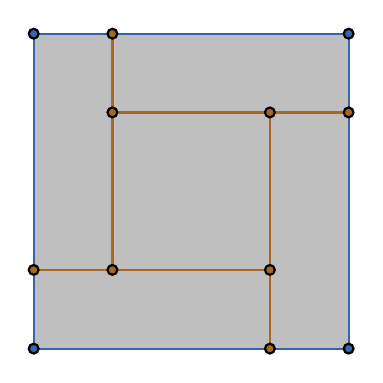
\begin{tikzpicture}[thick]
  \coordinate (p0) at (-2,-2);
  \coordinate (p1) at (2,-2);
  \coordinate (p2) at (2,2);
  \coordinate (p3) at (-2,2);
  \filldraw[fill=lightgray,draw=c0] (p0) -- (p1) -- (p2) -- (p3) -- cycle;%
  \node[point=c0] (m0) at (p0) {};
  \node[point=c0] at (p1) {};
  \node[point=c0] at (p2) {};
  \node[point=c0] at (p3) {};
  \coordinate (a0) at (-2,-1);
  \coordinate (a1) at (1,-1);
  \coordinate (a2) at (1,-2);
  \coordinate (a3) at (1,1);
  \coordinate (a4) at (2,1);
  \coordinate (a5) at (-1,1);
  \coordinate (a6) at (-1,2);
  \coordinate (a7) at (-1,-1);
  \draw[c1] (a0)--(a1);
  \draw[c1] (a2)--(a3);
  \draw[c1] (a4)--(a5);
  \draw[c1] (a6)--(a7);
  %%%
  \begin{scope}[shift={(-1.3,1)}]\sights\end{scope}
  \begin{scope}[shift={(-1,0.5)},rotate=90]\sights\end{scope}
  \begin{scope}[shift={(-1,-1.3)},rotate=90]\sights\end{scope}
  %%
  \begin{scope}[shift={(1,-1)},rotate=270]\sights[p1][q1][r1][c2!20!black]\end{scope}
  \begin{scope}[shift={(1.06,-.721)},rotate=250]\sights[p2][q2][r2][c2!40!black]\end{scope}
  \begin{scope}[shift={(1.2929,-.5858)},rotate=225]\sights[p3][q3][r3][c2!60!black]\end{scope}
  \begin{scope}[shift={(1.655,-.717)},rotate=200]\sights[p4][q4][r4][c2!80!black]\end{scope}
  \begin{scope}[shift={(2,-1)},rotate=180]\sights[p5][q5][r5][c2!100!black]\end{scope}
  %%
  %% \draw plot [smooth] coordinates {(q1)(q2)(q3)(q4)(q5)};
  \begin{scope}[shift={(0,0)},rotate=0]\crv\end{scope}
  \begin{scope}[shift={(-3,-2)},rotate=90]\crv\end{scope}
  \begin{scope}[shift={(0,0)},rotate=180]\crv\end{scope}
  \begin{scope}[shift={(3,2)},rotate=270]\crv\end{scope}
  %%
  \node[point=c1] (n0) at (a0) {};
  \node[point=c1] (n1) at (a1) {};
  \node[point=c1] (n2) at (a2) {};
  \node[point=c1] (n3) at (a3) {};
  \node[point=c1] (n4) at (a4) {};
  \node[point=c1] (n5) at (a5) {};
  \node[point=c1] (n6) at (a6) {};
  \node[point=c1] (n7) at (a7) {};
\end{tikzpicture}
\end{document}
